\section{Denoise Diffusion Probabilistic Models (DDPMs)}


\subsection{Diffusion Models (DMs)}

We previously talked about GANs, VAEs, and their variants (VQ-VAE, VQ-GAN). Diffusion models are also probabilistic models that define a non-linear mapping from latent variables to the observed data. Like variational autoencoders, they approximate the data likelihood using a lower bound. Diffusion models are easy to train and can produce very high-quality images compared to GANs.

A diffusion model consists of two main components: an encoder which takes a data sample $x$ and maps it through a series of intermediate latent variables $z_1, ..., z_T$, and a decoder which reverses this process, until it creates a sample image. The mappings are stochastic rather than discrete (the transformation between the latent variables involve some randomness).

% TODO: Explain LDMs
In the next section, we will take a closer look at DDPMs, which is subclass of DMs. Another class of DMs is called Latent Diffusion Models (LDMs) \cite{ldm}. 


\subsection{DDPMs}

Denoise Diffusion Probabilistic Models (DDPMs) \cite{ddpm} are a class of diffusion models that are trained to denoise images. In training phase, a dataset of images is fed to the model and DDPMs add noise to input image (it can be thought of as adding random pixel values to the input) in multiple steps (the intermediate latent variables $z_i$), unti the final result is pure noise (which will converge to the noise distribution). Then the model is trained to remove the noise and reconstruct the original image. The denoising process is called 'reverse diffusion' or reverse step and the noising process is called 'forward diffusion' or forward step. The forward diffusion step is denoted as $q(x_t | x_{t-1})$ and the reverse diffusion step is denoted as $p_\theta (x_{t-1} | x_t)$ (figure \ref{fig:ddpm_process}).

Because the addition of noise is a known stochastic process, all the learned parameters are in the decoder (the generator).



\begin{figure}
    \centering
    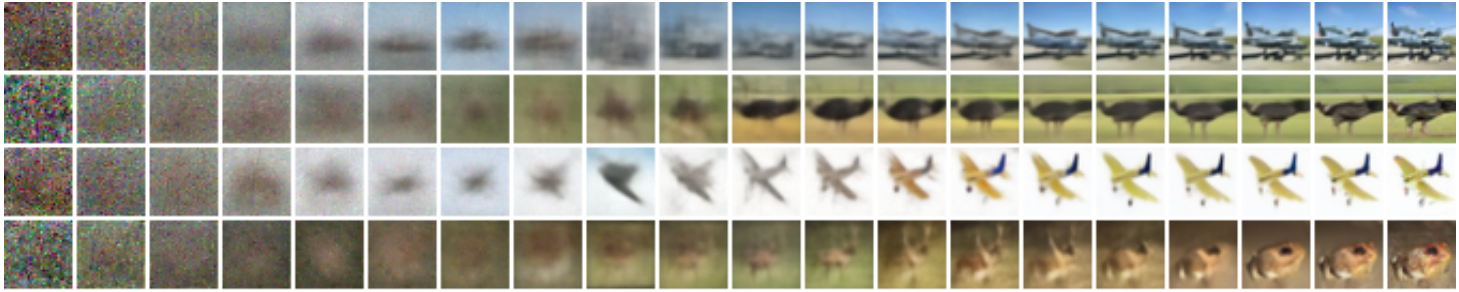
\includegraphics[width=1\textwidth]{images/diffusion_models/ddpm_denoise.png}
    \caption{Progressive generation (left to right) of unconditional CIFAR10 dataset in DDPM \cite{ddpm}.}
\end{figure}


\begin{figure}
    \centering
    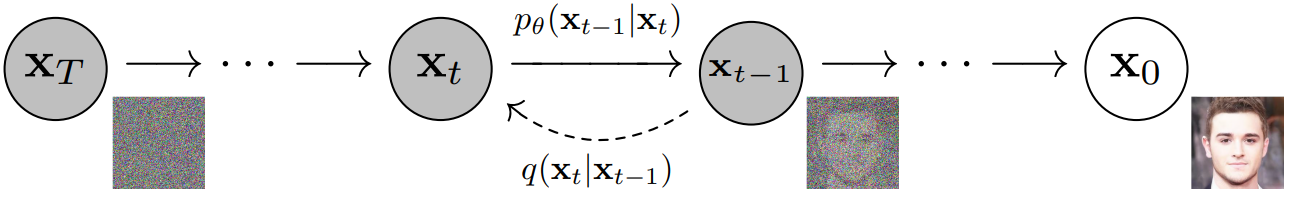
\includegraphics[width=1\textwidth]{images/diffusion_models/ddpm_process.png}
    \caption{A graph representing the forward and reverse diffusion process in DDPMs \cite{ddpm}. The next step (either in forward or reverse diffusion) depends conditionally on the previous steps ($p_\theta (x_{t-1} | x_t)$ and $q(x_t | x_{t-1})$).}
    \label{fig:ddpm_process}
\end{figure}



\subsection{Encoder}

The forward diffusion process maps a data image $x$ through a series of intermediate variables $z_1, ..., z_T$ with the dimension as $x$ according to the following recursion:

\begin{equation}
    \begin{aligned}
    \mathbf{z}_1 &= \sqrt{1 - \beta_1} \cdot \mathbf{x} + \sqrt{\beta_1} \cdot \epsilon_1, \\
    \mathbf{z}_t &= \sqrt{1 - \beta_t} \cdot \mathbf{z}_{t-1} + \sqrt{\beta_t} \cdot \epsilon_t \quad \forall \, t \in \{2, \ldots, T\}
    \end{aligned}
\end{equation}

At each step $i \in {1, 2, ..., t, t+1, ..., T}$, $e_i$ is a noise vector drawn from a standard normal distribution. 
